%%
%% Copyright 2007, 2008, 2009 Elsevier Ltd
%%
%% This file is part of the 'Elsarticle Bundle'.
%% ---------------------------------------------
%%
%% It may be distributed under the conditions of the LaTeX Project Public
%% License, either version 1.2 of this license or (at your option) any
%% later version.  The latest version of this license is in
%%    http://www.latex-project.org/lppl.txt
%% and version 1.2 or later is part of all distributions of LaTeX
%% version 1999/12/01 or later.
%%
%% The list of all files belonging to the 'Elsarticle Bundle' is
%% given in the file `manifest.txt'.
%%

%% Template article for Elsevier's document class `elsarticle'
%% with harvard style bibliographic references
%% SP 2008/03/01
%%
%%
%%
%% $Id: report01_prl.tex,v 1.3 2011/01/11 17:34:41 teerola Exp $
%%
%%
\documentclass[preprint,authoryear,review]{elsarticle}

%% Use the option review to obtain double line spacing
%% \documentclass[authoryear,preprint,review,12pt]{elsarticle}

%% Use the options 1p,twocolumn; 3p; 3p,twocolumn; 5p; or 5p,twocolumn
%% for a journal layout:
%% \documentclass[final,authoryear,1p,times]{elsarticle}
%% \documentclass[final,authoryear,1p,times,twocolumn]{elsarticle}
%% \documentclass[final,authoryear,3p,times]{elsarticle}
%% \documentclass[final,authoryear,3p,times,twocolumn]{elsarticle}
%% \documentclass[final,authoryear,5p,times]{elsarticle}
%% \documentclass[final,authoryear,5p,times,twocolumn]{elsarticle}

%% if you use PostScript figures in your article
%% use the graphics package for simple commands
%% \usepackage{graphics}
%% or use the graphicx package for more complicated commands
%% \usepackage{graphicx}
%% or use the epsfig package if you prefer to use the old commands
%% \usepackage{epsfig}

%% The amssymb package provides various useful mathematical symbols
%\usepackage{amssymb}

%
% OWN PACKAGES AND DEFINITIONS

\usepackage{paralist}

\graphicspath{{resources/}}

% math
\usepackage{amsmath}

% For nice PDF
\usepackage{times}
\usepackage{array}
\usepackage{pdfpages}

% new subfig format
%\usepackage[caption=false,font=normalsize,labelfont=sf,textfont=sf]{subfig}
\usepackage{subfig}

\usepackage[english]{babel} % For fixing the tilde problem https://bugs.launchpad.net/ubuntu/+source/texinfo/+bug/526974

% For commenting
\usepackage{color}
\newcommand\newnotecommand[3]{%
  \newcommand#1[1]{{\color{#3}\footnote{{\color{#3}#2:} ##1}}}}
\newnotecommand\joni{Joni}{red}
\newnotecommand\anders{Anders}{blue}

\usepackage[pagebackref=true,breaklinks=true,letterpaper=true,colorlinks,bookmarks=false]{hyperref}

\usepackage{multirow}
\usepackage{graphicx}
%\usepackage{graphicx}
%\usepackage[tight]{subfigure}
%\usepackage{amsmath}
%\usepackage{algorithmic} % for writing nice algorithms

%%
%% DEFINITION OF ALGORITHM ENVIRONMENT
%\newtheorem{alg}{Algorithm}
%\long\def\@makealgocaption#1#2{\vskip 2ex \small
%  \hbox to \hsize{\parbox[t]{\hsize}{{\bfseries #1.} #2}}}
%\newcounter{algorithm}
%\def\thealgorithm{\@arabic\c@algorithm}
%\def\fps@algorithm{tbp}
%\def\ftype@algorithm{4}
%\def\ext@algorithm{lof}
%\def\fnum@algorithm{Algorithm \thealgorithm}
%\def\algorithm{\let\@makecaption\@makealgocaption\@float{algorithm}}
%\let\endalgorithm\end

%% The amsthm package provides extended theorem environments
%% \usepackage{amsthm}

%% The lineno packages adds line numbers. Start line numbering with
%% \begin{linenumers}, end it with \end{linenumbers}. Or switch it on
%% for the whole article with \linenumbers after \end{frontmatter}.
\usepackage{lineno}

%% natbib.sty is loaded by default. However, natbib options can be
%% provided with \biboptions{...} command. Following options are
%% valid:

%%   round  -  round parentheses are used (default)
%%   square -  square brackets are used   [option]
%%   curly  -  curly braces are used      {option}
%%   angle  -  angle brackets are used    <option>
%%   semicolon  -  multiple citations separated by semi-colon (default)
%%   colon  - same as semicolon, an earlier confusion
%%   comma  -  separated by comma
%%   authoryear - selects author-year citations (default)
%%   numbers-  selects numerical citations
%%   super  -  numerical citations as superscripts
%%   sort   -  sorts multiple citations according to order in ref. list
%%   sort&compress   -  like sort, but also compresses numerical citations
%%   compress - compresses without sorting
%%   longnamesfirst  -  makes first citation full author list
%%
%% \biboptions{longnamesfirst,comma}

% \biboptions{}

\journal{Pattern Recognition Letters}

%\usepackage[usenames,dvipsnames]{color}
\newcommand{\commentNK}[1]{{\bf NK: #1}}

\begin{document}


\linenumbers

\begin{frontmatter}

%% Title, authors and addresses

%% use the tnoteref command within \title for footnotes;
%% use the tnotetext command for the associated footnote;
%% use the fnref command within \author or \address for footnotes;
%% use the fntext command for the associated footnote;
%% use the corref command within \author for corresponding author footnotes;
%% use the cortext command for the associated footnote;
%% use the ead command for the email address,
%% and the form \ead[url] for the home page:
%%
%% \title{Title\tnoteref{label1}}
%% \tnotetext[label1]{}
%% \author{Name\corref{cor1}\fnref{label2}}
%% \ead{email address}
%% \ead[url]{home page}
%% \fntext[label2]{}
%% \cortext[cor1]{}
%% \address{Address\fnref{label3}}
%% \fntext[label3]{}

\title{A comparison of local feature detectors and descriptors by intra-class repeatability and matching}

%% use optional labels to link authors explicitly to addresses:
%% \author[label1,label2]{<author name>}
%% \address[label1]{<address>}
%% \address[label2]{<address>}

\author[addrlutk]{Jukka~Lankinen}
\ead{Jukka.Lankinen@lut.fi}
\author[addrcovil]{Anders~Glent~Buch}
\ead{anbu@mmmi.sdu.dk}
\author[addrlutk]{Ville~Kangas}
\ead{Ville.Kangas@lut.fi}
\author[addrtut]{Joni-Kristian~K\"am\"ar\"ainen\corref{cor1}}
\ead{joni.kamarainen@tut.fi}
\cortext[cor1]{Corresponding author. Tel.: +358 40 5794605} 
\author[addrcovil]{Norbert~Kr\"uger}
\ead{norbert@mmmi.sdu.dk}

%\address[addrlut]{Machine Vision and Pattern Recognition Laboratory (MVPR),
%Department of Information Technology, 
%Lappeenranta University of Technology (LUT) %, P.O. Box 20, FIN-53851 Lappeenranta, Finland 
%(\url{http://www2.it.lut.fi/mvpr/})}

% Heikki: Pitäisikö siis olla MVPR:n osoite tämän laitoksen sijaan (\url{http://www.it.lut.fi})}? Näin muutin
%
%\address[addrlutk]{LUT Kouvola Unit, Kouvola, Finland}%, Lappeenranta
\address[addrlutk]{Lappeenranta University of Technology (LUT), LUT Kouvola, Finland}%, Lappeenranta
\address[addrcovil]{M{\ae}rsk McKinney M{\o}ller Institute, University of Southern Denmark, Denmark}%, Lappeenranta
\address[addrtut]{Department of Signal Processing, Tampere University of Technology, Finland}

%\address[addrtut]{Department of Automation Science and Engineering, Tampere
%University of Technology, P.O. Box 692, FIN-33101 Tampere, Finland}

%\lasse{Active or passive voice?}

%\lasse{Use either long (for example, that is, \ldots) or short (e.g.,
%i.e., \ldots) forms.}

%\lasse{Check the use of acronyms and initialisms.}


\begin{abstract}
Intuitive and easily interpretable local feature detector and descriptor
%repeatability and matching
performance measures and evaluation protocols were introduced
in~\cite{MikTuySch:2005,MikSch:2005}. They, however,
measured performances in wide baseline settings that do not correspond
to object class detection and recognition problems where the
detectors and descriptors are popular tools. This limitation has been
recognised and several ad~hoc evaluations reported.
This work extends the original performance
measures to the case of multiple examples of object classes and with our
novel framework we compare state-of-the-art detectors and descriptors.
%with object class datasets.

Our results from the detector comparison verify the wide baseline findings:
SIFT and SURF provide the most repeatable local regions between
instances of object classes. The detector differences are marginal and
in the descriptor comparison, the total number of detected regions
turned out to be more important giving preference to the Hessian-affine
detector. The most striking result, however, was the performance
collapse of all descriptors in intra-class matching---only a few
matches on average were found as compared to hundreds of matches in the
original works. This result
%The poor
%intra-class matching performance
indicates that even the best available descriptors
can be inadequate for large scale object classification
purposes.
%This finding supports
%the recent trend where other approaches, such as dense sampling, have been
%adopted and also motivates further investigation on local feature descriptors. 
%% At
%%first, that was our major conclusion from the descriptor evaluation where
%%descriptors paired with the Hessian-affine detector performed the best - a
%%finding already pointed out by \cite{NowJurTri:2006}:
%%``the more the better''. As a striking result, however,
Moreover, we found out that by using multiple best matches, even as few as
2-5, descriptor matching performance can be significantly improved. This
is particularly evident with the new performance measure proposed:
coverage-N (the number of images with at least N correct matches).

%Our findings indicate, that in large scale object classification,
%other than interest point based approaches, such as dense sampling,
%should be advocated, and novel object classification tailored local
%region descriptors should be developed or descriptor matching should
%utilise multiple matches.
%
%\commentNK{I feel this is a bit jumping to conclusions. It would be better in my view to extend the description of the actual problem you have spotted and given evidence for and then be very careful about the conclusions that might(!) be drawn.}

%Our results indicate, that an alternative claim to the Nowak et al. can be
%made: it is possible to perform well in visual class matching using a
%smaller number of local features and a smaller codebook by utilising
%multiple alternative assignments of local features -
%``less is more''.
\end{abstract}

\begin{keyword}
Feature detector \sep feature descriptor \sep local feature \sep object class detection
%% keywords here, in the form: keyword \sep keyword

%% MSC codes here, in the form: \MSC code \sep code
%% or \MSC[2008] code \sep code (2000 is the default)

\end{keyword}

\end{frontmatter}

% \linenumbers

%------------------------------------------------------------------------- 
%
\section{Introduction}
%
The problems of local image feature detection and description often occur
in computer vision where point correspondences between images are needed.
Solutions should tolerate illumination changes, zoom, blur and other
often encountered distortions. This is the case in many
applications, such as in wide-baseline matching (\cite{TuyGoo:2004}), robot
localisation (\cite{SeLowLit:2002}) and image stitching for panoramic
views (\cite{BroLow:2003}). In these, the correspondences are sought
between different views of the same scene and the evaluations by
\cite{MikTuySch:2005} and \cite{MikSch:2005} help to select the
most suitable method. Another popular application is visual object
classification (VOC), where objects in images should be identified.
In this case, the evaluations by Mikolajczyk et al.
are not
directly applicable, since the repeatability and matching performances
were computed for multiple views of a same object (scene) instead of
a set of object class examples.

Various methods have been proposed for detecting interest
points/regions and to construct descriptors for detected
regions, most of which are designed with a different application in mind.
\cite{MikTuySch:2005}
and \cite{MikSch:2005} evaluated and
compared the most popular detectors and descriptors. The detectors
were evaluated by their repeatability ratios and total number of 
correspondences over several view points and with various
imaging distortion types. The descriptors were evaluated by their matching
rates for the same views.
More adequate comparisons related to the
object classification task
have been reported by \cite{ZhaMarLaz:2006} and
\cite{MikLeiSch:2005}, but in these works
the evaluation was tied to a single methodological approach, namely
visual Bag-of-Words (BoW). In this work, we evaluate state-of-the-art
detectors and descriptors in the context of visual classification
and make the following contributions:
\begin{compactitem}
\item We extend the detector repeatability evaluation
  in~\cite{MikTuySch:2005} to intra-class repeatibility. Numbers of
  intra-class correspondences and repeatability rates are reported as
  the performance measures.
\item We extend the descriptor matching evaluation in~\cite{MikSch:2005} to
  the case of object classes.
  The intra-class match counts and rates are reported as the performance measures.
\item We propose {\em match coverage} as an alternative performance measure for descriptor evaluation: {\em coverage-N} measures how many image pairs
  contain at least N descriptor matches. This measure reveals the proportion of images in which the matching is expected to succeed.
\item We compare the most popular detector and descriptor methods and their various
  implementations in our novel intra-class evaluation setting.
\item We extend the original descriptor performance measures to use K best matches (K=1 in the
  original work). As will be shown, this modification is important and allows for significant improvements for object class matching.
\item For the detectors we verify the earlier results of their ranking, but for the descriptors
  we report a striking finding that the average number of matches collapses from hundreds to only
  a few. A significant improvement can be achieved by counting more than the one best match, but
  still the number of matching regions can be too low for large scale classification problems.
\end{compactitem}

%\commentNK{The last point is most important and should be discussed in its consequences for the computer vision community.}

This work extends our preliminary work in \cite{LanKanKam:2012} by revising the
experiments with more accurate measures that directly correspond to the original works
by Mikolajczyk et al., introducing the coverage-N performance measure and, in
particular, providing two important findings: with object class instances the
number of matching regions is very low, only a few as compared to hundreds in the
original work, and significant improvement can be achieved by counting more than one,
even as few as 5, best matches.
%surprising results when multiple best matches are counted.
%While mainstream in object classification has adopted the result by
%\cite{NowJurTri:2006} - ``the more the better'' - and thus dense
%sampling is popular, our novel results indicate that methods utilising multiple matches
%may succeed equally well - ``less is more''.

%All data and source code will be made publicly available to facilitate development of
%better approaches for detecting and matching local regions between object class
%instances. \commentNK{This is a promise, better to point to a web-page.}

%
\subsection{Previous work}
%
%\commentNK{I feel that this section is a bit thin. It depends a bit how aggressively we want to play it. Then the arguments should be better prepared.}


We believe that the general evaluation principles in~\cite{MikSch:2005,MikTuySch:2005} also hold in
the context of visual object classes: 1) \textit{detectors which return the same object regions for class
examples are good detectors} -- detection repeatability; 2)
\textit{descriptors which match the same object regions between class examples are good descriptors} -- match count/ratio. We refer to these repeating and matching regions as
``category-specific landmarks''. Indeed, a successful outcome of the categorisation task is important
for the final application, and therefore \cite{ZhaMarLaz:2006} compared different
detectors and descriptors using a baseline BoW method. In the baseline method, codebooks are constructed from
the raw descriptors and then images are categorised according to their codebook histograms.
In their work, \cite{MikLeiSch:2005}
were more specific by measuring average precision of feature clusters to represent a single class,
entropy of spatial location distribution produced by a single cluster (ideally compact) and complementarity
of different detectors. Both evaluations are biased by
the selected BoW approach. In this work, we show how the original evaluation principles can 
be adopted to obtain quantitative performance in the general and intuitive forms used in the original
works and not tied to a specific approach.


%------------------------------------------------------------------------- 
%
\section{Comparison of Region Detectors}
%
A good interest point detector for object classification should detect local
points or regions at the same object-relative locations, ``object landmarks'', on every
class example.
This criterion is different from~\cite{MikTuySch:2005}
in the sense that we evaluate detectors over examples of different 
categories instead of changed and distorted views of same scenes. In our case, visual appearance
variation is expected to be much larger.

%
\subsection{Data\label{sec:data}}
%
The experiments were conducted using the categories in the popular VOC dataset, Caltech-101~\cite{FeiFerPer:2006}.
For compactness and clarity, the results are reported for the following ten categories which
represent well the overall performance variation: \textit{watch}, \textit{stop\_sign}, \textit{starfish},
\textit{revolver}, \textit{euphonium}, \textit{dollar\_bill}, \textit{car\_side},
\textit{airplanes}, \textit{Motorbikes} and \textit{Faces\_easy}. The foreground areas,
included in the Caltech-101 ground truth data, were used to mask out interested points detected
on backgrounds.
Affine correspondences between the category examples were established
by manually annotating 5-12 landmarks per category and estimating the pair-wise image transformations
using the direct linear transform (\cite{HarZis:2003}). Example images with landmarks are shown
in Fig.~\ref{fig:affine_example1}.
%
For this experiment we used repeatedly 25 random pairs of images from each category (tot. of 500 images).
%each detector is run for all 500 images and then comparisons
%of features between image pairs are done, using the same methods as in
%~\cite{MikTuySch:2005}.
\begin{figure}[h]
\begin{center}
\subfloat{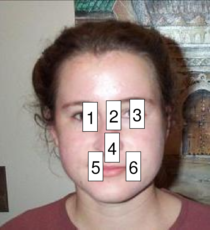
\includegraphics[height=0.16\linewidth]{resources/lm/lm_examples_cat01_img01.png}}
\subfloat{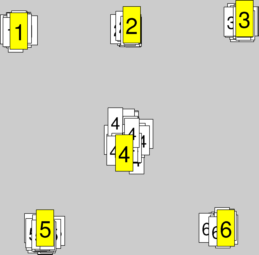
\includegraphics[height=0.16\linewidth]{resources/lm/lm_cat01.png}}~
\subfloat{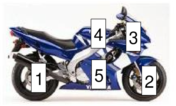
\includegraphics[height=0.16\linewidth]{resources/lm/lm_examples_cat02_img07.png}}
\subfloat{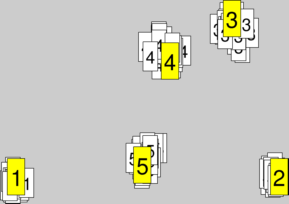
\includegraphics[height=0.16\linewidth]{resources/lm/lm_cat02.png}}\\
\subfloat{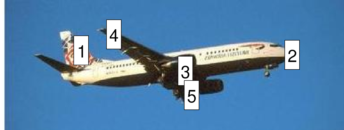
\includegraphics[height=0.1\linewidth]{resources/lm/lm_examples_cat03_img08.png}}
\subfloat{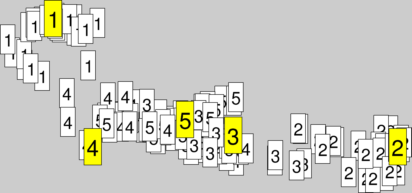
\includegraphics[height=0.1\linewidth]{resources/lm/lm_cat03.png}}~
\subfloat{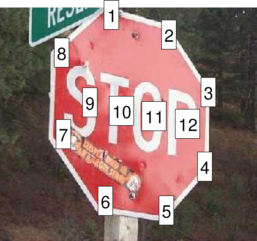
\includegraphics[height=0.16\linewidth]{resources/lm/lm_examples_cat09_img01.png}}
\subfloat{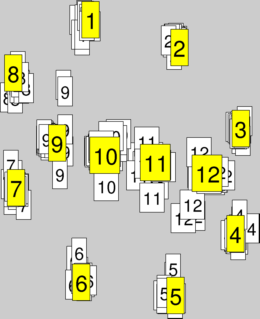
\includegraphics[height=0.16\linewidth]{resources/lm/lm_cat09.png}}\\
\subfloat{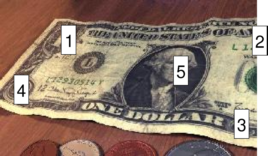
\includegraphics[height=0.12\linewidth]{resources/lm/lm_examples_cat05_img04.png}}
\subfloat{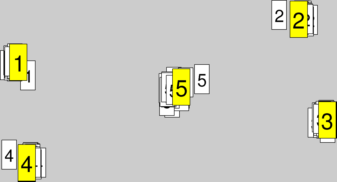
\includegraphics[height=0.12\linewidth]{resources/lm/lm_cat05.png}}~
\subfloat{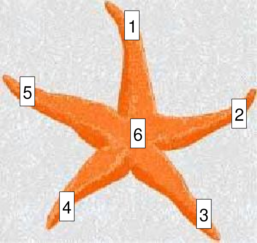
\includegraphics[height=0.14\linewidth]{resources/lm/lm_examples_cat08_img02.png}}
\subfloat{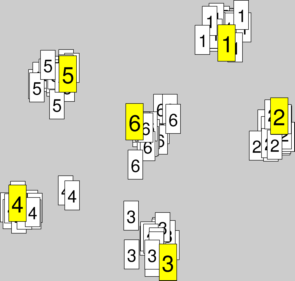
\includegraphics[height=0.14\linewidth]{resources/lm/lm_cat08.png}}\\
\subfloat{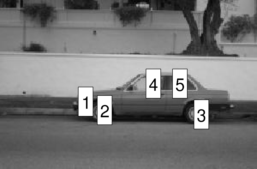
\includegraphics[height=0.14\linewidth]{resources/lm/lm_examples_cat04_img02.png}}
\subfloat{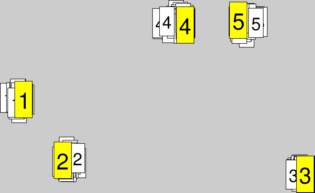
\includegraphics[height=0.14\linewidth]{resources/lm/lm_cat04.png}}~
\subfloat{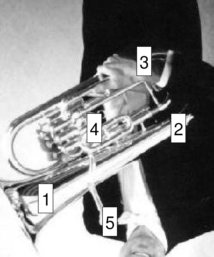
\includegraphics[height=0.14\linewidth]{resources/lm/lm_examples_cat06_img02.png}}
\subfloat{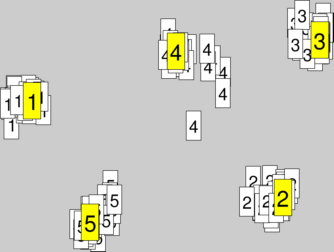
\includegraphics[height=0.14\linewidth]{resources/lm/lm_cat06.png}}\\
\subfloat{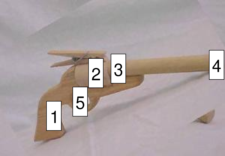
\includegraphics[height=0.14\linewidth]{resources/lm/lm_examples_cat07_img10.png}}
\subfloat{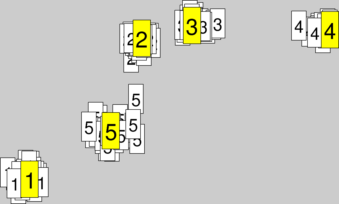
\includegraphics[height=0.14\linewidth]{resources/lm/lm_cat07.png}}~
\subfloat{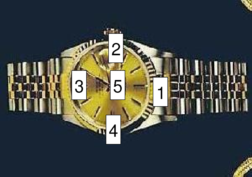
\includegraphics[height=0.12\linewidth]{resources/lm/lm_examples_cat10_img18.png}}
\subfloat{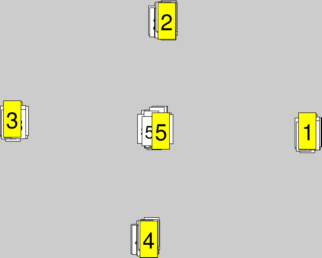
\includegraphics[height=0.12\linewidth]{resources/lm/lm_cat10.png}}
\caption{Selected object classes with annotated landmarks and their ``canonical spaces'' where all landmark tuples are projected onto the random example (denoted by the yellow tags). The two standard deviations of the image diagonal normalised projection errors are (from left to right and top to bottom):
0.0158,
0.0297,
0.1701,
0.0460,
0.0304,
0.0373,
0.0194,
0.0641,
0.0486, and
0.0177.\label{fig:affine_example1}}
\end{center}
\end{figure}

%
\subsection{Region detectors}
%
Our comparison includes nine publicly available and popular detectors: 
three implementations of Hessian-affine, two implementations of Difference-of-Gaussian (DoG),
SURF, Laplacian-of-Gaussian, Harris-Laplace and MSER. %\anders{Zhao's Hessian-Laplace \textit{hesslap-vireo} is grouped here as one of the three Hessian-affine, but is it actually affine-invariant?}
% Actually it is ``nearly'' affine-invariant, but let's avoid too many details ;-)

The Hessian-affine detector (\cite{MikSch:2002}) performed well in the comparison 
by~\cite{MikTuySch:2005}, and therefore we 
included both Mikolajczyk's original 
(\textit{hessaff-alt}) and a more recent implementation (\textit{hessaff}),
and an alternative implementation by~\cite{lip-vireo} (\textit{hesslap-vireo}).
%with
%a slightly different algorithm.
%
Our set of ``fast detectors'' consisted of Difference-of-Gaussian (DoG) by~\cite{Low:2004} (\textit{sift}),
Zhao's implementation of DoG (\textit{dog-vireo}) and speeded-up robust features
(SURF) by~\cite{BayEssTuy:2008} (\textit{surf}).
%
In addition, Zhao's implementation of Laplacian-of-Gaussian (LoG) (\textit{log-vireo}),
Harris-Laplace (\textit{harlap-vireo}) and Maximally Stable Extremal Regions (MSER) by~\cite{MatChuUrb:2002} (\textit{mser}) were included. \textit{*-vireo} implementations were from Zhao's
Lip-vireo toolkit (\url{http://code.google.com/p/lip-vireo/}), \textit{hessaff} and
\textit{hessaff-alt} were Mikolajczyk's implementations available at
\url{http://featurespace.org}, \textit{surf} is available at the authors' web site
and \textit{mser} and \textit{sift} in the popular VLFeat library (\url{http://vlfeat.org}).

There are many more detectors, but the aforementioned represent the best
performed in the earlier studies and those which performed well in our preliminary
tests. All experiments were conducted using the available implementations and their default parameters.

%
\subsection{Performance measures and evaluation}
%
For the detector performance evaluation, we adopted the test protocol in~\cite{MikTuySch:2005}.
Interest points are first extracted from images. The interest points detected inside the object area (Caltech-101 foreground) are selected for the evaluation.
%
For each image pair, points from the first image are projected onto the second image.
The projection is an affine transformation estimated using the annotated landmarks.
The landmarks projected on a randomly selected example of each category
are demonstrated in Fig.~\ref{fig:affine_example1} with the
two standard deviations corresponding to the 95\% error distributions.
%Only features covered by
%both images are considered, though in this case practically all the features
%fulfill that requirement.
Interest regions are described by 2D ellipses and
a sufficient overlap of fixed scale ellipses in both images is accepted as a correct correspondence.
The number and rate of the correspondences for each detector is of interest. A detector performs well
if the total number is large and also reliably if the ratio is high.
We used the parameter settings
from~\cite{MikTuySch:2005}: 40\% overlap threshold and normalisation of the ellipses to
the radius of 30 pixels. %\commentNK{This is a bit unclear for me but experts might now}

The reported performance numbers are the average number of corresponding regions between
image pairs and the repeatability rate, i.e. the ratio between the corresponding 
regions and the total number of detected regions.

\subsection{Results}
Results are gathered in Fig.~\ref{fig:results1}.
%From the results we can see that when comparisons are done over different
%examples of images contained by a class, values drop quite drastically, but
%still median repeatability rates are well above the zero, except for the
%extremely challenging airplanes class.
There are significant differences between the different categories.
Dollar bill and stop sign are generally the easiest, as expected due to
lower variation in their visual appearance, while the airplanes, car side views and revolvers are
the most difficult. For the airplanes this
can be explained by the fact that one of the landmarks is placed on the wing resulting in
3D pose changes instead of 2D affinities.
The numbers for all categories are by order of magnitude smaller than for the fixed
scenes in~\cite{MikTuySch:2005}, being tens of correspondences instead of hundreds of
them.
%\commentNK{What do we learn from that? Categorization is quite a different problem requiring probably features with higher level of abstraction}
%
\begin{figure}[h]
\begin{center}
\subfloat[]{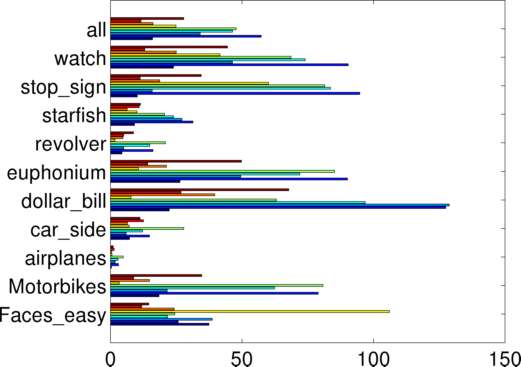
\includegraphics[width=0.49\linewidth,height=0.4\linewidth]{resources/ville_results/detcor-avg.png}}
\subfloat[]{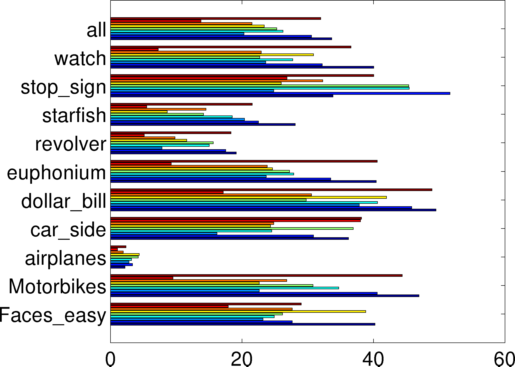
\includegraphics[width=0.49\linewidth,height=0.4\linewidth]{resources/ville_results/detrep-avg.png}}

\subfloat[]{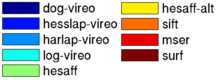
\includegraphics[width=0.3\linewidth]{resources/ville_results/detector-legend.png}}
\subfloat[]{\scriptsize
\begin{tabular}{|l|l|l|}
\hline
\textbf{Method} & \textbf{Avg \# of corr.} & \textbf{rep. rate}\\
\hline
\textit{dog-vireo}     & 16.0 & 33.7\%\\
\textit{hesslap-vireo} & 57.4 & 30.6\%\\
\textit{harlap-vireo}  & 34.2 & 20.3\%\\
\textit{log-vireo}     & 46.5 & 26.3\%\\
\textit{hesaff}        & 47.8 & 25.3\%\\
\textit{hesaff-alt}    & 25.0 & 23.4\%\\
\textit{sift}          & 16.2 & 21.5\%\\
\textit{mser}          & 11.7 & 13.8\%\\
\textit{surf}          & 27.9 & 32.0\%\\
\hline
\end{tabular}}
\caption{Detector evaluation: 
(a) average number of corresponding regions,
%\textit{dog-vireo}: 16.0;
%\textit{hesslap-vireo}: 57.4;
%\textit{harlap-vireo}: 34.2;
%\textit{log-vireo}: 46.5;
%\textit{hesaff}: 47.8;
%\textit{hesaff-alt}: 25.0;
%\textit{sift}: 16.2;
%\textit{mser}: 11.7;
%\textit{surf}: 27.9;
(b) repeatability rates,
%\textit{dog-vireo}: 33.7\%;
%\textit{hesslap-vireo}: 30.6\%;
%\textit{harlap-vireo}: 20.3\%;
%\textit{log-vireo}: 26.3\%;
%\textit{hesaff}: 25.3\%;
%\textit{hesaff-alt}: 23.4\%;
%\textit{sift}: 21.5\%;
%\textit{mser}: 13.8\%;
%\textit{surf}: 32.0\%;
(c) colour coding of the detectors, and (d) overall results table.\label{fig:results1}}
\end{center}
\end{figure}
%\begin{figure}[h]
%\begin{center}
%\subfloat[]{\includegraphics[width=0.9\linewidth]{resources/detcor-median.png}}
%\subfloat[]{\includegraphics[width=0.9\linewidth]{resources/detrep-median.png}}
%\caption{(a) median number of corresponding regions, (b) median repeatability rate.\label{fig:results1_median}}
%\end{center}
%\end{figure}
%

The following three methods have good repeatability ratio: hesslap-vireo,
dog-vireo and surf. 
%\commentNK{Can we argue why?}
They frequently detect regions from the same relative positions from
all examples. On the other hand, classification methods require a sufficient number of
correspondences to form a discriminative description. In this sense,
hesslap-vireo ($\approx$ hessaff), is very good. Its repeatability rate is
the third best (30\%) and it provides more correspondences (57) on average. Dog-vireo
($\approx$ sift) has the best repeatability (33\%), but its average number of correspondences (16) can
be too low for large scale categorisation. Surf has the second best repeatability (32\%) and
it provides 27 correspondences on average. Since the repeatability rates are very similar for the three
best, the selection is based on the preferred number of correspondences.
Surprisingly, the MSER detector, which was among the top performers in Mikolajczyk's study, was now clearly the worst.%\anders{I think I can explain why: MSERs are covariant regions formed by a closed contour around some local shape in the image, with the constraint that the color difference be high between the inside and the outside of the contour. Think of e.g. a letter as the local MSER. Thus, MSERs are highly covariant in wide baseline settings, since the same shape can be found quite stably. Here, however, the local shape appearance varies between object class examples, and the completely degrades the performance of MSER. In other words, MSERs are much better for recognition of the same local shape than they are for classification of shapes.} % that is very true, and for artificial objects, in general, /Joni
It is furthermore interesting that Zhao's recent implementations 
provide better results than the original methods (hesslap-vireo $=$ hessaff/hessaff-alt
and dog-vireo $=$ sift).
%\commentNK{'dog-vireo $\leftrightarrow$ sift' is unclear to me} ). %This needs to be taken in account when choosing a feature detector since different
%implementations of the same region detector provide noticeably different
%detection results.

As a summary, the recent implementations: hesslap-vireo, hessaff
and log-vireo perform best, $\approx50$ corresponding regions on average with
25-30\% repeatability rate. The numbers are however clearly smaller than for
different view points of a same scene / object (\cite{MikTuySch:2005}).% \commentNK{Can you argue why that is?}


%------------------------------------------------------------------------- 
%
\section{Comparison of Local Region Descriptors}
%
A good region descriptor for the object classification problem should be
discriminative to match only correct regions, but also tolerate
small appearance variation between category examples. These requirements are
general for feature extraction in computer vision and image
processing. The descriptor performances were obtained in the original
work (\cite{MikSch:2005}) by computing statistics of the correct and false
matches. In the case of classification, the descriptor matches are expected to
be weaker due to increased variance in the visual appearance of regions.
For example, scooters and road bikes are both in the
Caltech-101 motorbikes category, but their pair-wise similarity
is much weaker than between two scooters or two road bikes.
%Moreover, there is natural variation in the spatial configurations
%of the regions (constellation deformation).
%Therefore, we
%need to tailor the original method to cope with these two sources
%of variation.

We also propose an alternative measure, {\em coverage}, which
measures the number of images ``covered'' with at least the given number of correspondences N (coverage-N). 
This complements the original evaluation criteria, since coverage
reports for how many image pairs at least a required number N of
correct matches have been found (a single or few pairs of a huge number
of matches do not affect the measure).


%To evaluate the performance of local descriptors selected we simply
%count matches and calculate statistics out of them. Test protocol used in
%\cite{MikSch:2005} is not suitable for this evaluation because the task for
%descriptors is not exactly the same. As we are searching for matches between
%various items in the same object category, the number of matches we can
%assume to be found is significantly lower than if we would try to find
%matches between two images taken at the same scene.

%Although the task of finding matches is not easy, in many cases several 
%matches can be found. If a few matches for an image pair is enough, depends on
%the application. Combining matches of several methods is also a possibility
%that can increase the number of found matches especially when there are
%different kinds of source images in use.

%We use term ``coverage'' to show in how many of the image pairs descriptor
%matches were found. Coverage-n then shows the pairs where $ n $ or more
%matches are found. It can reveal some properties of descriptors as some
%have ability to obtain a few matches even in very challenging image pairs 
%that with most descriptors no matches can be found. It is important to note that
%used detector affects this as it determines the spatial locations in the 
%image that descriptors are calculated for.

%
\subsection{Available descriptors}
%
Out of the many available descriptors we wanted to test the most
frequently used and best performing. In~\cite{MikSch:2005}, the SIFT
detector by~\cite{Low:2004} and its extension, the gradient location
and orientation histogram (GLOH) (\cite{MikSch:2005}), obtained the best
results.
%GLOH is here omitted as its proper use would require a training set.
A more recent descriptor SURF by \cite{BayEssTuy:2008},
%As with detectors, descriptors for this evaluation were selected using the
%existing knowledge and preliminar tests about their performance. As the 
%chosen detector also has impact on the performance of the descriptor, some 
%descriptors occur in the descriptor evaluation more than once combined with 
%various detectors.
%SIFT ~\cite{Low:2004} is the most widely used descriptor and two
%implementations of it are evaluated combined with several detectors. GLOH
%is a slightly different version of SIFT proposed in ~\cite{MikSch:2005}.
%SURF,
besides being very fast detector, is a robust descriptor and
conceivably more tolerant to at least moderate amount of noise than
SIFT. In most works, these three descriptors are considered. Moreover, we selected one ``traditional''
descriptor based on multiresolution Gabor filters, which resembles the responses
of oriented filters (steerable filters),
%\commentNK{I believe that this term 'steerable filters' is misguiding here. Why not just say 'Gabor wavelets'.},
included in the original work, but omitted ever since due to
limited discriminative power.
However, in this context,
the better generalisation and weaker specificity can be advantageous.
For simplicity we replaced the steerable
filters with a similar bank of Gabor filters which have been successful in face
detection (\cite{WisFelKru:1997}). %\commentNK{I believe that citation is misleading. Daugman has first applied Gabor wavelets, Wiskott et all have first applied them to face recognition and Granlund has invented them. Any of these three would be a better citation.}
%similar works (steerable filters), but
%which was not among the best performers.

%For the SIFT descriptor, we selected two implementations, the
%original by~\cite{Low:2004} (\textit{sift}) and a more recent by
%\cite{lip-vireo} (\textit{sift-vireo}). The orientation filter
%descriptor (\textit{lin.filters}) was our own implementation.
%%For GLOH we used the
%%implementation by Mikolajczyk (\textit{gloh}) and
%For SURF the
%implementation by its original authors (\cite{BayEssTuy:2008})
%(\textit{surf}) was used. Ideally, we should combine these descriptors with all
%the three best detectors, but the following best combinations were
%selected according to our preliminary tests: 1)
%\textit{hesslap-vireo+sift-vireo} ($\approx$ hesaff+sift), 2)
%\textit{dog-vireo+sift-vireo} ($\approx$ sift+sift), 3)
%\textit{hesaff+sift}, 4) \textit{surf+surf}, 5) \textit{hesaff+lin.filters} and
%6) \textit{sift+sift}. It should be noted, that the available executables
%do not allow arbitrary combinations.
For the descriptor comparison we selected the best performing detectors, the
Hessian derivatives being the most important. Based on the preliminary tests, we
report the results for \textit{hessaff+sift} (FeatureSpace implementations),
\textit{mser+sift} (VLFeat implementations), \textit{surf+surf}
(\cite{BayEssTuy:2008} implementations), \textit{sift+sift}
(VLFeat) and \textit{hessaff+gabor} (FeatureSpace detector and our own
descriptor implementations).

\subsection{Performance measures and evaluation\label{sec:descrperformance}}

%\commentNK{I would take out the first two sentences, since it is an unnecessary detour.} 
%In our previous work in~\cite{LanKanKam:2012}, we replaced the Mikolajczyk's
%matching criterion (the ellipse overlap error used in the detector evaluation),
%with a simpler and less strict ellipse centroid distance threshold. That,
%however, lead to over-optimistic results and therefore for this work
%we adopted the original criterion from~\cite{MikSch:2005}.
At first, descriptors are computed for
all detected regions (foreground only). Images are processed
pair-wise and best matches for the regions are sought by computing
one-to-all distances and selecting the closest match. It is worth noting
that the rule proposed in~\cite{Low:2004} for discarding ``bad regions''
(ratio between the first and the second best is less than $1.5$) must
not be used with object classes since it would produce virtually no matches
at all. This can be explained by the fact that matches are
never as good as in the wide baseline case. We used the maximum ellipse
overlap error $50\%$ from~\cite{MikSch:2005} for finding detector correspondences.
% (note that the detector evaluation
%used the more strict limit of $40\%$). \commentNK{Why?}
%This rule is default in many implementations, but it makes
%the matching performance collapse. %The rule discards outliers in the wide baseline case.
%%: if the distance to the second best match is below
%%Next, due to a large number of false and a small
%%number of correct matches, we adopted the rule proposed 
%%in~\cite{Low:2004}: if the distance to the second best match is below
%%$1.5$ times the distances to the best, the match between these points
%%is removed as incorrect.

%Our spatial verification stage differs from~\cite{MikSch:2005} by
%being less strict since the original rule provides only a few matches for the 
%most pairs. In the original rule, the regions were described by
%ellipses, and for the spatial verification the ellipses were projected onto
%each other using the estimated affine transformation. If a sufficient 
%overlap occurred for the ellipses, then the match was accepted.
%In our case, however, the categories have natural variation in
%their spatial structure. This natural variation
%cannot be exactly encoded into affine transformation and
%therefore the matches are not exact even for the ground truth landmarks as demonstrated in
%Fig.~\ref{fig:affine_example1}. The two standard deviations vary
%between 0.0158 (Faces\_easy) and 0.0641 (euphonium). The airplanes category is an outlier due to the one no%n-2D landmark on the wing tip (0.1701).  However, for ellipse overlap
%computation, even a small difference in the ellipse centroid may have
%an enormous effect to the overlap area~\cite{MikTuySch:2005}. The
%configuration is sufficiently affine over views of a same planar scene, but
%for VOC evaluation we needed to replace the ellipse overlap rule with a distance
%threshold between the ellipse centroids. For resolution independence, the distances were normalised with
%the image diagonal and in our evaluation we discarded
%matches if the distance was greater than $0.05$. This threshold covers the two
%standard deviations of the ground truth landmarks and over 95\% of the landmarks are within 
%this distance.

Our performance numbers are the average number of matches and median
%\commentNK{Wouldn't it make more sense to then use also the median for the detectors?}
number of matches. The median is used to suppress the effect of
several too well matching pairs (a same person, identical
stop signs, etc.) For applications, it is also important to know how many matches
are guaranteed to be found, and thus,
%This can vary between images and is not uniform if the difference between the
%average and median is large. Thus,
we also report ``coverage'' numbers.
%, i.e. a 
%number of image pairs for which at least N matches have been found
%({\em coverage-N}). \anders{I don't think we need to re-explain the coverage term here, so we could remove the ``, i.e...'' part from this sentence.}

%
\subsection{Results}
%
The data for this experiment were the same.
The average and median number of matches are shown in
Fig.~\ref{fig:results2}. %\anders{This figure still needs rearrangement of elements.}
%\joni{Anders, please remove the labels from figures and save them as a single image (similar to sub-fig c) from the old version), also limit the x-axis to 50 or 30 for clarity, moreover, add correct values to the table}\anders{There's now an attempt to meet this. Let me know if you want it changed!}
% CVPR2012/ICPR interpretations removed since completely wrong
For most of the classes, the mean and median numbers are very low, average median being
0-2 for all detector-descriptor combinations,
which clearly is not adequate since higher level processing stages of
visual classification cannot compensate for that.
Category-wise coverages are reported in Fig.~\ref{fig:results2_2}.
At least one match can be found on average from 19 out of 25
(\textit{hesaff-sift}). For five
matches, the number drops from 19 to 8 ($32\%$ of pairs) and for
ten matches it is only 4 ($16\%$). 
The best results were obtained for the stop signs, dollar bills and
faces, but the overall performance is poor.
The best discriminative methods could still learn to detect these
categories, but it is difficult to imagine naturally emerging
``common codes'' for other classes except the stop signs, faces and
dollar bills.
It is surprising that the best detectors were able to provide
50 repeatable regions on average, but only a few descriptors
between these regions match.
% (even with the less strict ellipse
%overlap error threshold).
The main conclusion of these results is that all descriptors perform
poorly in matching similar regions between class examples.


% It is no surprise, that in state-of-the-art
%codebook (bag-of-features) based VOC methods, the poor matching has been compensated, for
%example, by variants of ``soft assignment''~\cite{AgaTri:2008,TuySch:2007} or multiple features are enforce%d to the same code
%using spatial co-location or co-occurrence information instead of the feature similarity~\cite{LeiEttSch:2008}. 
%
\begin{figure}[h]
\begin{center}
%\subfloat[]{\includegraphics[width=0.9\linewidth]{resources/mean-all.png}}\\
%\subfloat[]{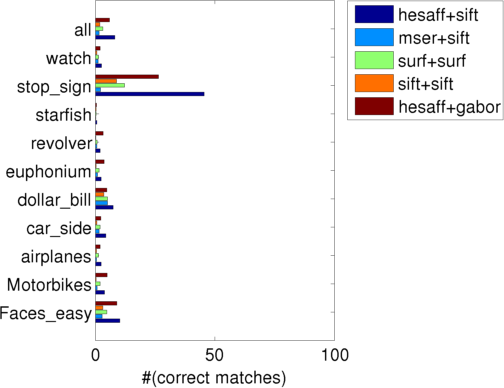
\includegraphics[width=0.49\linewidth]{resources/anders_results/results_descriptor/mean-all-b1.png}}
\subfloat[]{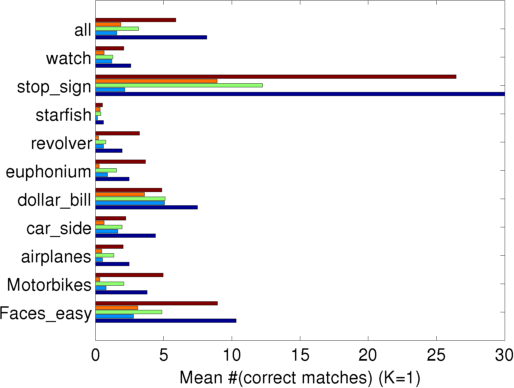
\includegraphics[width=0.49\linewidth]{resources/anders_results/2012.11.26_results_descriptor/mean-all-b1.png}}
%
%\subfloat[]{\includegraphics[width=0.9\linewidth]{cvpr2011/resources/median-all.png}}\\
%\subfloat[]{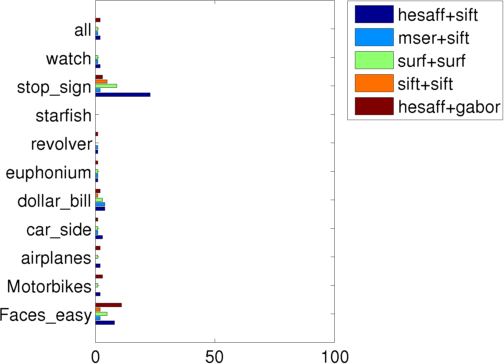
\includegraphics[width=0.49\linewidth]{resources/anders_results/results_descriptor/median-all-b1.png}}
\subfloat[]{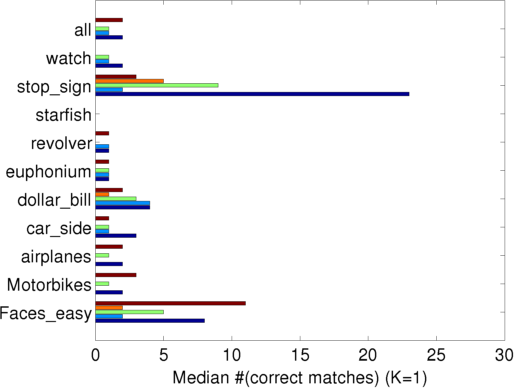
\includegraphics[width=0.49\linewidth]{resources/anders_results/2012.11.26_results_descriptor/median-all-b1.png}}

%\subfloat[]{\includegraphics[width=0.8\linewidth]{cvpr2011/resources/descriptor-legend.png}}\\
%\subfloat[]{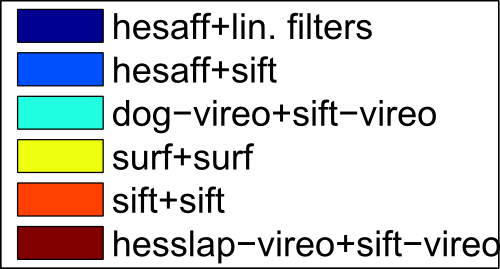
\includegraphics[width=0.3\linewidth]{resources/jukka_results/sg_descriptor/colors.png}}\hfill
\subfloat[]{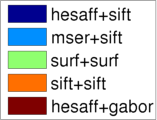
\includegraphics[width=0.2\linewidth]{resources/anders_results/2012.11.26_results_descriptor/mean-all-b1-legend.png}}\hfill
\subfloat[]{\scriptsize
% VILLES RESULTS FROM HIS MSTHESIS
%%\begin{tabular}{|l|l|l|}
%%\hline
%%\textbf{Method} & \textbf{Avg \#} & \textbf{Med \#}\\
%%\hline
%%\textit{sift+sift}                & 2.6 & 1.0\\
%%\textit{hesaff+gloh}              & 6.3 & 0.0\\
%%\textit{surf+surf}                & 2.7 & 1.0\\
%%\textit{hessaff+sift}             & 6.3 & 0.0\\
%%\textit{dog-vireo+sift-vireo}     & 2.6 & 1.0\\
%%\textit{hesslap-vireo+sift-vireo} & 3.4 & 0.5\\
%%\hline
%%\end{tabular}}
% JUKKAS RESULTS FROM CVPR2012 NOW W/O LOWES CUT-OUT RULE
%\begin{tabular}{|l|l|l|}
%\hline
%\textbf{Method} & \textbf{Avg \#} & \textbf{Med \#}\\
%\hline
%\textit{hesaff+lin.filt.}         & 58.9 & 39.0\\
%\textit{hessaff+sift}             & 66.1 & 46.0\\
%\textit{dog-vireo+sift-vireo}     & 18.7 & 15.0\\
%\textit{surf+surf}                & 12.3 & 9.0\\
%\textit{sift+sift}                &  9.5 & 6.0\\
%\textit{hesslap-vireo+sift-vireo} & 30.9 & 22.0\\
%\hline
%\end{tabular}}
% ANDERSES RESULTS NOW W/O LOWE RULE BUT USING ELLIPSE OVERLAPS
% AGB: TAKEN FROM resources/anders_results/2012.11.26_results_descriptor/mean-median-all-b1-table.png
\begin{tabular}{|l|l|l|}
\hline
\textbf{Method} & \textbf{Avg \#} & \textbf{Med \#}\\
\hline
\textit{hessaff+sift}             & 8.2 & 2\\
\textit{hessaff+gabor}            & 5.9 & 2\\
\textit{mser+sift}                & 1.6 & 1\\
\textit{surf+surf}                & 3.2 & 1\\
\textit{sift+sift}                & 1.9 & 0\\
\hline
\end{tabular}}
\caption{Descriptor evaluation: (a) average number of matches per class,
%\textit{sift+sift}: 2.6;
%\textit{hesaff+gloh}: 6.3;
%\textit{surf+surf}: 2.75;
%\textit{hessaff+sift}: 6.3;
%\textit{dog-vireo+sift-vireo}: 2.6;
%\textit{hesslap-vireo+sift-vireo}: 3.4;
(b) median,
%\textit{sift+sift}: 1.0;
%\textit{hesaff+gloh}: 0.0;
%\textit{surf+surf}: 1.0;
%\textit{hessaff+sift}: 0.0;
%\textit{dog-vireo+sift-vireo}: 1.0;
%\textit{hesslap-vireo+sift-vireo}: 0.5;
(c) colour coding of the method names, and
(d) overall results table.
\label{fig:results2}}
\end{center}
\end{figure}
%
\begin{figure}[h]
\begin{center}
%\subfloat[]{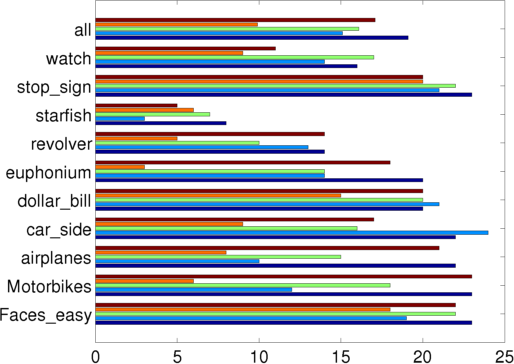
\includegraphics[width=0.42\linewidth]{resources/anders_results/results_descriptor/coverage-1-b1.png}}
%\subfloat[]{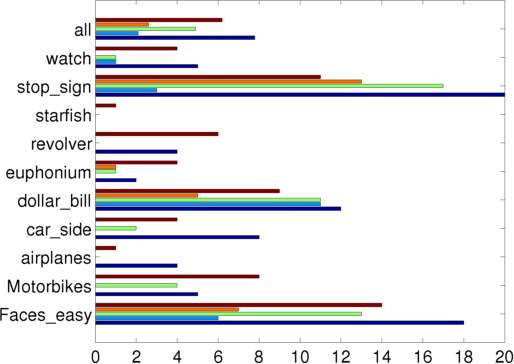
\includegraphics[width=0.35\linewidth,trim=70 0 0 0,clip=true]{resources/anders_results/results_descriptor/coverage-5-b1.png}}
%\subfloat[]{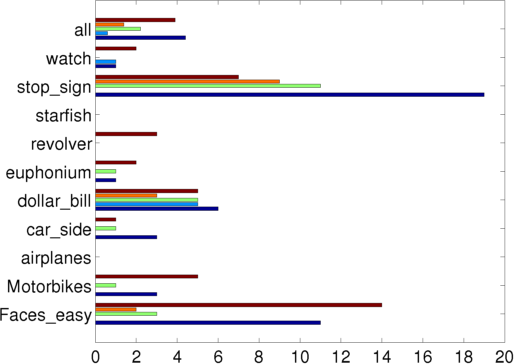
\includegraphics[width=0.35\linewidth,trim=70 0 0 0,clip=true]{resources/anders_results/results_descriptor/coverage-10-b1.png}}
\subfloat[]{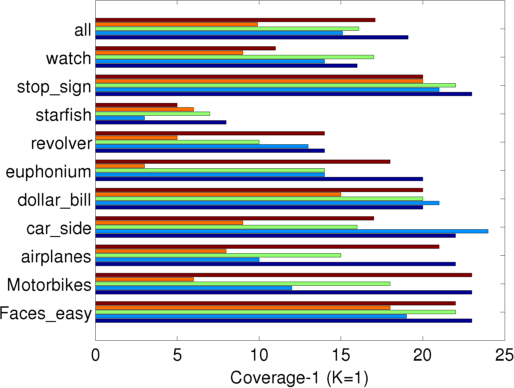
\includegraphics[width=0.435\linewidth]{resources/anders_results/2012.11.26_results_descriptor/coverage-1-b1.png}}
\subfloat[]{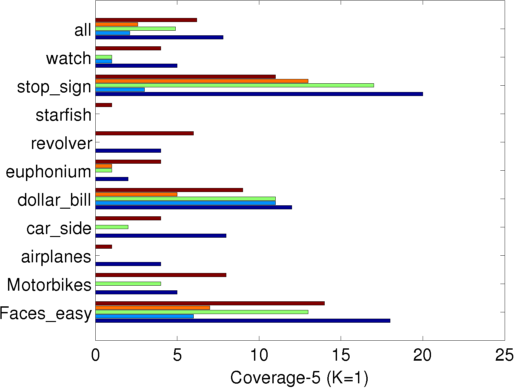
\includegraphics[width=0.35\linewidth,trim=80 0 0 0,clip=true]{resources/anders_results/2012.11.26_results_descriptor/coverage-5-b1.png}}
\subfloat[]{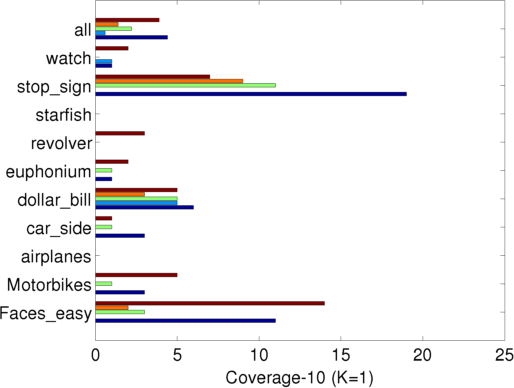
\includegraphics[width=0.35\linewidth,trim=80 0 0 0,clip=true]{resources/anders_results/2012.11.26_results_descriptor/coverage-10-b1.png}}
\caption{Descriptors evaluation: (a) coverage-1; (b) coverage-5; (c) coverage-10.\label{fig:results2_2}}
\end{center}
\end{figure}


%
\subsection{Beyond single best matches}
The descriptor results are disappointingly bad, but it is interesting to study whether
the poor matching can be compensated somehow. Our next experiment was motivated by the
soft assignments successfully used in classification methods utilising interest points
(e.g., \cite{AgaTri:2008,TuySch:2007}). It
also seems intuitively correct that the best matches are not always
correct between two different instances, and thus a few best
should be tested. We tested this hypothesis by counting matches correct if they
were within the K best and satisfied the overlap criterion. The coverage graphs
for varying $K$ are shown in Fig.~\ref{fig:coverage}. Increasing $K$ had a
clear positive effect on the performance. This is evident already in coverage-1 (at least one
match found between every pair), but especially the increase from 8 to 22 images for
 $K=5$ with coverage-5 (middle column in Fig.~\ref{fig:coverage}) and from 4 to 13 with
coverage-10 are significant improvements (\textit{hesaff-sift}).
Beyond $K=5$ performances still improve, but not as significantly anymore.
% started to saturate. \commentNK{I am not clear how I can see that}

%
\begin{figure*}
\begin{center}
%%\subfloat[]{\includegraphics[width=0.44\linewidth]{cvpr2011/resources/coverage-all.png}}\\
%%\subfloat[]{\includegraphics[width=0.24\linewidth]{cvpr2011/resources/coverage-5.png}}
%%\subfloat[]{\includegraphics[width=0.24\linewidth]{cvpr2011/resources/coverage-3.png}}
%%\subfloat[]{\includegraphics[width=0.24\linewidth]{cvpr2011/resources/coverage-2.png}}
%\subfloat[]{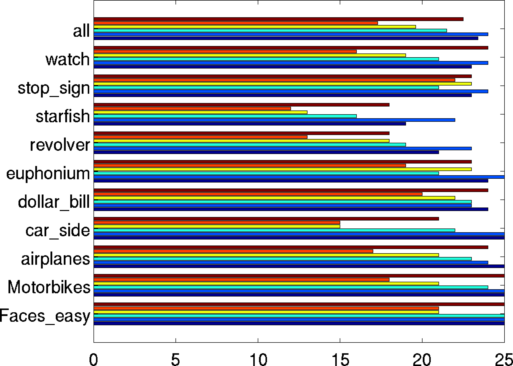
\includegraphics[width=0.45\linewidth,height=0.25\linewidth]{cvpr2011/resources/bestMatch/sg_descriptor/0.05/png/coverage-5-b1.png}} \hfill
%\subfloat[]{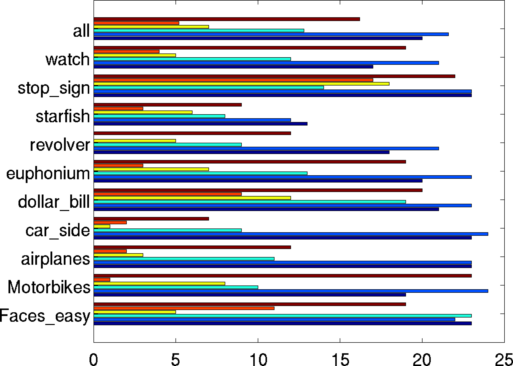
\includegraphics[width=0.45\linewidth,height=0.25\linewidth]{cvpr2011/resources/bestMatch/sg_descriptor/0.05/png/coverage-15-b1.png}}\\
%\subfloat[]{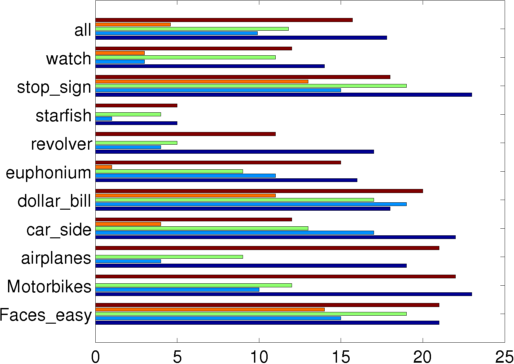
\includegraphics[width=0.45\linewidth,height=0.25\linewidth]{cvpr2011/resources/bestMatch/sg_descriptor/0.05/png/coverage-5-b5.png}} \hfill
%\subfloat[]{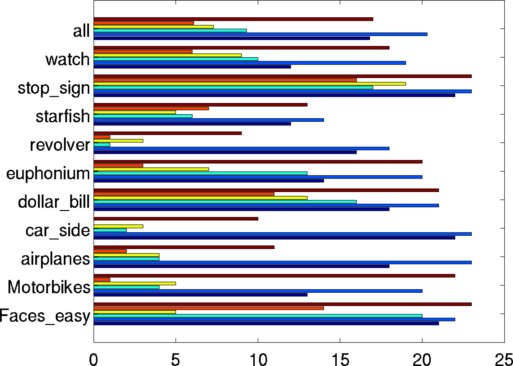
\includegraphics[width=0.45\linewidth,height=0.25\linewidth]{cvpr2011/resources/bestMatch/sg_descriptor/0.05/png/coverage-15-b5.png}}
%\subfloat{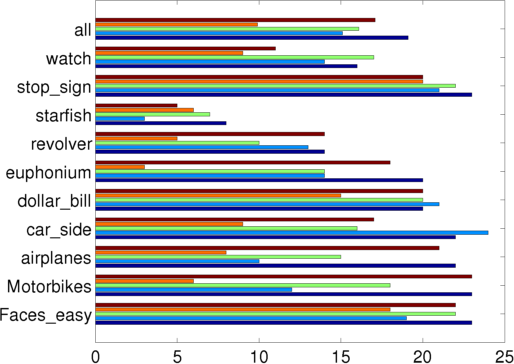
\includegraphics[width=0.42\linewidth]{resources/anders_results/results_descriptor/coverage-1-b1.png}}
%\subfloat{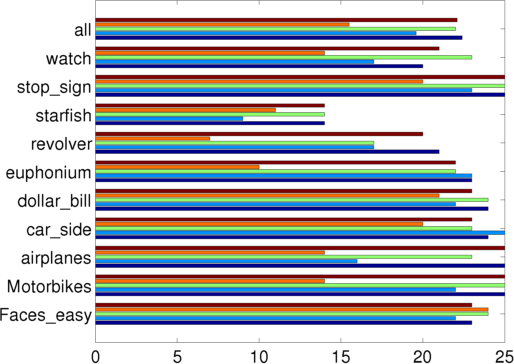
\includegraphics[width=0.35\linewidth,trim=70 0 0 0, clip=true]{resources/anders_results/results_descriptor/coverage-1-b5.png}}
%\subfloat{\includegraphics[width=0.35\linewidth,trim=70 0 0 0, clip=true]{resources/anders_results/results_descriptor/coverage-1-b10.png}}\\
%\subfloat{\includegraphics[width=0.42\linewidth]{resources/anders_results/results_descriptor/coverage-5-b1.png}}
%\subfloat{\includegraphics[width=0.35\linewidth,trim=70 0 0 0, clip=true]{resources/anders_results/results_descriptor/coverage-5-b5.png}}
%\subfloat{\includegraphics[width=0.35\linewidth,trim=70 0 0 0, clip=true]{resources/anders_results/results_descriptor/coverage-5-b10.png}}\\
%\subfloat{\includegraphics[width=0.42\linewidth]{resources/anders_results/results_descriptor/coverage-10-b1.png}}
%\subfloat{\includegraphics[width=0.35\linewidth,trim=70 0 0 0, clip=true]{resources/anders_results/results_descriptor/coverage-10-b5.png}}
%\subfloat{\includegraphics[width=0.35\linewidth,trim=70 0 0 0, clip=true]{resources/anders_results/results_descriptor/coverage-10-b10.png}}
\subfloat{\includegraphics[width=0.435\linewidth]{resources/anders_results/2012.11.26_results_descriptor/coverage-1-b1.png}}
\subfloat{\includegraphics[width=0.35\linewidth,trim=80 0 0 0, clip=true]{resources/anders_results/2012.11.26_results_descriptor/coverage-1-b5.png}}
\subfloat{\includegraphics[width=0.35\linewidth,trim=80 0 0 0, clip=true]{resources/anders_results/2012.11.26_results_descriptor/coverage-1-b10.png}}\\
\subfloat{\includegraphics[width=0.435\linewidth]{resources/anders_results/2012.11.26_results_descriptor/coverage-5-b1.png}}
\subfloat{\includegraphics[width=0.35\linewidth,trim=80 0 0 0, clip=true]{resources/anders_results/2012.11.26_results_descriptor/coverage-5-b5.png}}
\subfloat{\includegraphics[width=0.35\linewidth,trim=80 0 0 0, clip=true]{resources/anders_results/2012.11.26_results_descriptor/coverage-5-b10.png}}\\
\subfloat{\includegraphics[width=0.435\linewidth]{resources/anders_results/2012.11.26_results_descriptor/coverage-10-b1.png}}
\subfloat{\includegraphics[width=0.35\linewidth,trim=80 0 0 0, clip=true]{resources/anders_results/2012.11.26_results_descriptor/coverage-10-b5.png}}
\subfloat{\includegraphics[width=0.35\linewidth,trim=80 0 0 0, clip=true]{resources/anders_results/2012.11.26_results_descriptor/coverage-10-b10.png}}
%\subfloat[]{\includegraphics[width=0.33\linewidth]{resources/coverage-10-b5.png}}
\caption{Descriptor evaluation results using $K$ best matches. From left to right: $K=1, 5, 10$, respectively. From top down: coverage-1, coverage-5, coverage-10.
\label{fig:coverage}}
\end{center}
\end{figure*}

% JONI REMOVED THIS EXPERIMENT SINCE IT DOES NOT REALLY PROVIDE ANYTHING SIGNIFICANT NEW AND
% THE RESULTS ARE EVEN MORE DISAPPOINTING
%\subsection{Validation dataset}
%\joni{Anders: please, repeat the experiment with this data - it should only require
%downloading the data and the new image pair files}\anders{Done! However, I suggest removing the median data since it% is identically zero.}
%One possible explanation for the bad descriptor performance is the poor
%image quality of the most Caltech-101 categories. To study the effect of
%image quality, we collected our own data set, referred to as ``LUTMVPR-12''.
%The data set consist of 12 classes of
%which 6 are the same to Caltech-101 (watches,
%stop signs, revolvers, motorbikes, cars and airplanes). LUTMVPR-12 images
%are of good resolution and quality. The images were collected from Flickr and
%by taking photographs in the town centre. The results are shown
%in Fig.~\ref{fig:results_lut10_1}.
%The results are almost equal to the Caltech-101 results and therefore
%support the previous findings.
%\begin{figure}[h]
%\begin{center} % In both of these figures, X axis is limited to 0-20
%%\subfloat[]{\includegraphics[width=0.44\linewidth]{resources/ville_results/minna-mean-all.png}}
%%\subfloat[]{\includegraphics[width=0.44\linewidth]{resources/ville_results/minna-median-all.png}}
%\subfloat[]{\includegraphics[width=0.44\linewidth]{resources/anders_results/results_minna/mean-all-b1.png}}
%\subfloat[]{\includegraphics[width=0.44\linewidth]{resources/anders_results/results_minna/median-all-b1.png}}
%%\subfloat[]{\includegraphics[width=0.44\linewidth]{resources/ville_results/minna-coverage-all.png}}
%\caption{Descriptor evaluation for LUTMVPR-12: (a) average and (b) median
%number of matches per class.
%% (c) coverages for at least one match per class (coverage-1).
%%Coverage number corresponds to the total number of image pairs per class (the maximum is 10).
%\label{fig:results_lut10_1}}
%\end{center}
%\end{figure}
%
%\commentNK{I am a bit unsure about how to present the results. Figure \ref{fig:results_lut10_1} is empty. Also I fee%l - unless it is a standard data base - then more detail on the data (and in particular on the differences to Caltec%h) should be given.}


%------------------------------------------------------------------------- 
%
\section{Conclusions}
%
Our work provides important experimental findings contributing to
visual object classification research where interest point detectors
and descriptors have been a popular approach. We extended the easily
interpretable and intuitive interest point detector and descriptor
performance measures from~\cite{MikTuySch:2005} and~\cite{MikSch:2005},
repeatability and number of matches, to measure intra-class performance
using random pairs of object class examples. The most popular
detectors and descriptors were compared using the Caltech-101 data set.
% and
%the results verified using our own LUTMVPR-12 data set with the same
%categories, but much better image quality.

The best performing detectors, the Hessian derivatives particularly,
provide moderately large numbers of corresponding regions between object
class instances ($\approx50$). The most striking result, however, is
that the state-of-the-art descriptors cannot match these regions well (only
0-2 matches on average). The problem has been known for some time among
the most experienced researchers in the field,  but to the authors' best
knowledge our work provides the first explicit and quantitative results
supporting the fact. Our
results advocate more research on novel object class tuned descriptors and
alternative matching approaches. Many alternatives can already be found
from the existing literature, for example, enhanced codebook generation
with co-location and co-activation clustering (\cite{LeiEttSch:2008}) and
soft-assignment of descriptor codes (\cite{AgaTri:2008,TuySch:2007}).
Also the finding by \cite{NowJurTri:2006}---``the more the
merrier''---seems to apply in the case of object classification and gives
preference
to methods producing a large number of regions. This is already evident
in state-of-the-art where dense sampling has replaced interest points
(see the methods in \cite{pascal-voc-2012}). The dense sampling may have
problems with rotation and scale invariance, but to circumvent these
limitations the recently introduced idea of ``dense interest points''
(\cite{Tuy:2010}) can be further elaborated. Our future work will address
the problems of how to select better regions and how to match the
regions for improved object classification on a large scale.

%% References with bibTeX database:

\bibliographystyle{elsarticle-harv}
\bibliography{intraclass}

%% Authors are advised to submit their bibtex database files. They are
%% requested to list a bibtex style file in the manuscript if they do
%% not want to use elsarticle-harv.bst.

%% References without bibTeX database:

% \begin{thebibliography}{00}

%% \bibitem must have one of the following forms:
%%   \bibitem[Jones et al.(1990)]{key}...
%%   \bibitem[Jones et al.(1990)Jones, Baker, and Williams]{key}...
%%   \bibitem[Jones et al., 1990]{key}...
%%   \bibitem[\protect\citeauthoryear{Jones, Baker, and Williams}{Jones
%%       et al.}{1990}]{key}...
%%   \bibitem[\protect\citeauthoryear{Jones et al.}{1990}]{key}...
%%   \bibitem[\protect\astroncite{Jones et al.}{1990}]{key}...
%%   \bibitem[\protect\citename{Jones et al., }1990]{key}...
%%   \harvarditem[Jones et al.]{Jones, Baker, and Williams}{1990}{key}...
%%

% \bibitem[ ()]{}

% \end{thebibliography}

\end{document}

%%
%% End of file `elsarticle-template-harv.tex'.
